\documentclass[sigconf,review]{acmart}
\microtypesetup{expansion=false}
\usepackage{array}
\setcopyright{none}
\acmConference[Preprint]{Preprint}{November 2026}{}
\acmYear{2026}
\copyrightyear{2026}

\settopmatter{printacmref=false}
\renewcommand\footnotetextcopyrightpermission[1]{}
\begin{document}
\setlength{\emergencystretch}{3em}

\title{Who Rewrites the Loop?}
\subtitle{Human versus Agent Authorship in the Recursive Self-Improvement of Open-Source Agent Harnesses}

\author{Haoyi Xiong}
\affiliation{\institution{Independent Researcher}\country{}}

\author{Yekun Chai}
\affiliation{\institution{Independent Researcher}\country{}}

\begin{abstract}
Agent harnesses---the loops, context managers, tool interfaces, and sandboxes that turn a language model \citep{chen2021} into a working software agent---are now among the fastest-moving artifacts in open-source software. Claims of recursive self-improvement (RSI) imply that agents increasingly rewrite the very harnesses they run on. Yet there is little repository-level evidence about \emph{who} changes which part of a harness, and whether such changes survive review. We report a mining study of 20 open-source agent harnesses and runtimes, covering 135,331 pull requests (PRs) created between May 2025 and November 2026. We introduce a three-tier attribution scheme (autonomous agent, co-authored/assisted, no explicit marker) and a pointcut taxonomy that separates the core loop (L1), context and memory (L2), tools and sandbox (L3), evaluation and infrastructure (L4), product surface (L0), and documentation (LD). We combine a rule engine over all PRs with a 7,205-PR detail sample and a 120-PR model-assisted adjudication. Explicitly agent-attributable PRs are 5.2\% of decided PRs (T1 2.87\%, T2 2.33\%). Their merge odds are lower (Mantel--Haenszel OR 0.709, 95\% CI 0.682--0.738), but the effect reverses in repositories that treat agents as first-class contributors. Autonomous agents are concentrated in L4 and L0: only 13.2\% touch the core loop, versus 26.0\% for unmarked PRs, and only 15.8\% are structural changes, versus 22.9\%. Co-authored PRs, by contrast, touch the core at 28.8\% and are structural at 30.2\%. We read this as empirical support for a \emph{protected-variation} discipline in harness engineering: agents are delegated to stable variation points, while humans retain the stable core. The findings reframe RSI as maintenance-layer self-improvement rather than architectural self-authorship, and identify repository governance---not agent brand---as the strongest predictor of agent contribution outcomes.\end{abstract}

\ccsdesc[500]{Software and its engineering~Software evolution}
\ccsdesc[300]{Software and its engineering~Software design engineering}
\ccsdesc[300]{General and reference~Empirical studies}

\keywords{mining software repositories, agent harness, design patterns, software evolution, recursive self-improvement}

\maketitle

\section{Introduction}

An \emph{agent harness} is the software layer that makes a language model act: it owns the turn loop, assembles context, exposes tools, enforces permissions, executes commands in a sandbox, and decides when to stop. In 2025--2026 the harness became a product category of its own---Codex, Gemini CLI, Claude Code, OpenCode, Cline, Continue, Goose, OpenHands, SWE-agent, and a growing set of agent SDKs. It also became a substrate for a stronger claim: that agents can improve the harness that runs them, producing a recursive self-improvement (RSI) loop \citep{lehman1980,godfrey2008}.

The claim is plausible but under-specified. A repository can contain agent-authored documentation, tests, adapters, and even core-loop refactors, and each implies a different kind of self-improvement. Existing studies of AI-assisted development measure productivity \citep{peng2023,ziegler2022}, code quality \citep{barke2023}, or benchmark success \citep{jimenez2024,yang2024,wang2025}. They do not tell us which architectural layer agent changes reach, whether those changes survive peer review, or whether the same agent behaves differently across repositories. These are mining-software-repositories (MSR) questions, and they require a taxonomy of the artifact before they can be answered.

Two recent Google systems make the design question concrete. OO-Harness evolves a hierarchy of executable harness classes through inheritance and a router, reporting up to 15\% absolute improvement over a base harness on long-horizon benchmarks \citep{li2026ooharness}. Harness$^2$ applies two connected levels of recursion---task-level harness refinement and harnessing-level experience accumulation---and reports gains of up to 11.5 points on WorkBuddy-Bench, 4.5 on JobBench, and 11.8 on LAB \citep{xu2026harness2}. Both are benchmark studies of what a harness can become; neither observes who actually rewrites harnesses in open-source repositories, which layer those changes reach, or whether they survive review. That is the gap this paper fills.

This paper asks three questions. \textbf{RQ1}: Who authors changes to a harness, and how do agent-attributed PRs fare in review? \textbf{RQ2}: Which architectural layer do agent changes target, and is there a ``no-go zone'' around the core control flow? \textbf{RQ3}: How do harness patterns diffuse across repositories, and do agents carry that diffusion?

We study 20 repositories spanning four interaction regimes---CLI/terminal, IDE-integrated, autonomous/async SWE, and framework/SDK runtime---over an 18.6-month window. We collect 151,509 PRs, exclude 16,178 dependency, release, and mirror-bot PRs, and retain 135,331. All retained PRs receive metadata-level attribution; 7,205 receive file-, commit-, and review-level detail; 120 are independently adjudicated by a model that sees the PR content but not the rule output.

Our contributions are:
\begin{itemize}
\item a \emph{three-tier attribution} scheme that separates autonomous agent PRs from co-authored/assisted PRs and from the unmarked baseline, and reports the limitations of each;
\item a \emph{pointcut taxonomy} for harness internals (L1--L4) with two contrast layers (L0 product surface, LD documentation) and an explicit generated-code layer, validated at 3.4\% unclassified line volume;
\item repository-level evidence that agent contribution is \emph{layer-selective}: autonomous agents are concentrated in tests, infrastructure, UI, and documentation, while the stable core remains human-owned;
\item evidence that co-authored PRs are the channel through which agents reach structural change, touching the core more often than either autonomous agents or unmarked human PRs;
\item a descriptive account of harness-pattern diffusion (skills/rules, context compaction, sub-agents, checkpoints, MCP) with explicit left-censoring caveats.
\end{itemize}

The rest of the paper is organized as follows. Section~\ref{sec:background} reviews harnesses, object-oriented design patterns, and MSR background. Section~\ref{sec:rq} states the research questions. Section~\ref{sec:design} describes the sample, attribution, taxonomy, and collection. Section~\ref{sec:measurement} describes labeling and statistics. Section~\ref{sec:results} reports results. Section~\ref{sec:discussion} discusses implications for design patterns and RSI. Section~\ref{sec:threats} addresses validity, and Section~\ref{sec:conclusion} concludes.

\section{Background and Related Work}
\label{sec:background}

\subsection{The harness as a software artifact}

We define a harness along four responsibilities. The \emph{core loop} (L1) decides what the agent does next: it runs the turn cycle, maintains the state machine, schedules sub-agents, retries failures, and decides termination. \emph{Context and memory} (L2) decide what the agent sees and remembers: system prompts, compaction and truncation, retrieval and code indexing, session persistence, and rule/skill definitions. \emph{Tools and environment} (L3) decide what the agent can do and what it is allowed to do: tool and MCP interfaces, shell/browser/file executors, patch application, permission checks, sandboxing, model-provider adapters, and external protocols. \emph{Evaluation and infrastructure} (L4) supports development: tests, benchmarks, CI, telemetry, and tracing. We add two contrast layers: product surface (L0: webviews, TUI rendering, websites, examples) and documentation (LD). Generated code, lockfiles, minified bundles, and patches are separated into a non-analyzed GEN layer because they inflate line counts without representing design decisions.

This decomposition is deliberately close to the concerns that object-oriented design (OOD) already names. The core loop is a \emph{template method} or \emph{state} machine; context management is a \emph{strategy} plus a \emph{memento}; tool adapters are \emph{adapters} and \emph{bridges}; permissions are a \emph{proxy} or \emph{decorator}; and sub-agent scheduling is a \emph{mediator} or \emph{coordinator}. The harness is therefore a fertile site for asking whether classical design patterns still organize change when the implementer may be an agent.

\subsection{Object-oriented design, patterns, and protected variation}

Design patterns codify recurring solutions to recurring design problems \citep{gof1994}. The deeper principle behind many of them is Parnas's information hiding: modules should conceal design decisions likely to change \citep{parnas1972}. In architectural terms, a pattern defines a \emph{pointcut} (where a concern applies), a \emph{contract} (what must remain true), and a \emph{variation seam} (what may be replaced) \citep{fielding2000,posa2000}. The ``protected variation'' heuristic---encapsulate what varies, keep the stable interface closed---is the design rule we will use to interpret our results.

Harness engineering has rediscovered these rules under new names. ``Bring your own model'' is a strategy/adapter seam. ``Deferred tool loading'' is a lazy proxy. ``Context compaction'' is a memento plus a policy. ``Sub-agent orchestration'' is a mediator. The POHE field guide~\footnote{\url{https://harness-pattern.github.io/pohe/}} catalogs 52 such candidate patterns and argues that a harness pattern is only useful if its pointcut, contract, permitted variation, test obligation, and negative control are explicit. Our taxonomy is the empirical counterpart: it asks which layer a change lands in, not which pattern a repository claims to implement.

OO-Harness \citep{li2026ooharness} is the closest design-side precedent. It treats a harness as a class hierarchy: an evolution agent creates specialized subclasses from execution records, and a router selects one at test time. This is inheritance and polymorphism applied to the harness itself, and it reports up to 15\% absolute improvement over a base harness. Our taxonomy is deliberately lower-level: we do not assume a class hierarchy, only that a change lands in a layer. The two views are complementary---OO-Harness asks how to organize variation, our study asks where variation is actually exercised in practice.

\subsection{Mining pull-based development}

GitHub's pull-based model has been studied extensively: contribution evaluation depends on social and technical signals \citep{tsay2014}, review is a distributed peer-review process \citep{rigby2008}, and repository mining has well-known promises and perils \citep{kalliamvakou2014,bird2009}. Prior work on open-source evolution establishes that change is concentrated in some modules and that architecture constrains who can change what \citep{mockus2002,herbsleb2003,nagappan2008}. Our study applies this lens to a new artifact and a new author type.

A growing body of work---much of it preliminary---uses bot accounts and co-author trailers to identify agent involvement on GitHub. What is missing is not evidence that agents open pull requests, but a layer-resolved account of what those requests change, how they fare in review, and whether the pattern is stable across repositories. Our taxonomy and three-tier attribution are designed to supply that account.

\subsection{Recursive self-improvement}

RSI denotes a system that improves the process by which it improves itself. In software, the observable proxy is an agent contributing to its own runtime. The proxy is imperfect: an agent may write tests for its harness without touching the loop, or a human may write code with an unmarked agent assistant. We therefore treat RSI as a \emph{spectrum of attribution and layer}, not a binary.

Recent work turns RSI from a slogan into an optimization loop. Harness$^2$ separates task-level recursion (edit the current harness without a ground-truth verifier) from harnessing-level recursion (distill edits into a reusable improvement harness), and reports gains across four model--harness configurations \citep{xu2026harness2}. OO-Harness instead evolves a population of harness classes and routes tasks to them \citep{li2026ooharness}. Both evaluate on benchmarks with frozen models. Our contribution is orthogonal: we measure the human--agent division of labor in the repositories where harnesses are actually maintained. The empirical question is not ``does RSI exist'' but ``how far up the stack does it reach, and under what governance does it survive review.''

\section{Research Questions}
\label{sec:rq}

\textbf{RQ1 (Attribution and contribution).} What share of harness PRs is explicitly agent-attributable, and how do agent-attributed PRs differ from unmarked PRs in merge rate, review activity, and revert rate? We expect agent PRs to merge less often if review acts as a quality filter, but we also expect repository-level heterogeneity.

\textbf{RQ2 (Pointcut and no-go zones).} Which architectural layers do agent PRs target? We test the \emph{no-go-zone} hypothesis: autonomous agents concentrate in low-coupling layers (tests, tool adapters, UI, docs) and rarely touch the core loop, permissions, or concurrency model. We also test the \emph{architectural-entropy} hypothesis: agent changes prefer local conditional patches over abstraction extraction.

\textbf{RQ3 (Diffusion and behavioral clusters).} Do harness patterns spread across repositories, and do agents carry the spread? We track six pattern families and cluster repository--tier behavior vectors to see whether ``agent fingerprints'' are stable across repositories or are a function of repository architecture.

\section{Study Design}
\label{sec:design}

\subsection{Sample}

We selected 20 repositories in four strata: CLI/terminal-native (6), IDE-integrated (3), autonomous/async SWE (5), and framework/SDK runtime (6). The sample intentionally includes same-lineage pairs---Cline/Roo-Code, Gemini CLI/Qwen Code, OpenHands/software-agent-sdk---to observe forking and migration effects. Table~\ref{tab:sample} lists the repositories and retained PR counts.

\begin{table*}[t]
\centering
\small
\caption{Sample. PR counts are retained PRs created 2025-05-01 to 2026-11-20 after excluding dependency, release, and mirror bots.}
\label{tab:sample}
\begin{tabular}{@{}llrr@{}}
\toprule
Stratum & Repository & Lang. & PRs \\
\midrule
CLI & openai/codex & Rust & 12,907 \\
    & google-gemini/gemini-cli & TS & 12,809 \\
    & QwenLM/qwen-code & TS & 10,406 \\
    & anomalyco/opencode & TS/Go & 29,658 \\
    & aaif-goose/goose & Rust/TS & 6,797 \\
    & Aider-AI/aider & Python & 710 \\
\midrule
IDE & cline/cline & TS & 7,018 \\
    & continuedev/continue & TS & 3,225 \\
    & RooCodeInc/Roo-Code & TS & 5,274 \\
\midrule
Autonomous & OpenHands/OpenHands & Py/TS & 6,915 \\
    & OpenHands/software-agent-sdk & Python & 4,088 \\
    & SWE-agent/SWE-agent & Python & 335 \\
    & SWE-agent/mini-swe-agent & Python & 700 \\
    & browser-use/browser-use & Python & 3,491 \\
\midrule
Framework & openai/openai-agents-python & Python & 3,507 \\
    & mastra-ai/mastra & TS & 15,300 \\
    & crewAIInc/crewAI & Python & 4,841 \\
    & langchain-ai/langgraph & Python & 3,140 \\
    & google/adk-python & Python & 2,914 \\
    & huggingface/smolagents & Python & 1,296 \\
\midrule
\multicolumn{3}{r}{Total} & 135,331 \\
\bottomrule
\end{tabular}
\end{table*}

\subsection{Unit, window, and exclusions}

The unit is a pull request targeting the default branch. The window is 2025-05-01 to 2026-11-20 (18.6 months). We exclude PRs authored by dependency and release bots, mirror bots (e.g., Copybara accounts), and PRs whose titles match release-version patterns. We retain agent-executed dependency migrations when the author is not a dependency bot. For merge-rate analysis we right-censor at 2026-09-21, giving each PR at least 60 days to merge.

The raw crawl yields 151,509 PRs; 16,178 are excluded, leaving 135,331. Of these, 110,469 are decided (merged or closed unmerged) by the cutoff. All 135,331 receive metadata-level attribution; 7,205 receive detail.

\subsection{Three-tier attribution}

Table~\ref{tab:tiers} defines the tiers. Tier~1 is deliberately conservative: a bot account, a bot author type, or an explicit statement that the PR was generated end-to-end by an AI. Tier~2 requires a positive artifact---a co-author trailer, a tool signature, or a structured ``AI-assisted: yes'' field. Tier~3 is the absence of any marker. We call Tier~3 the \emph{unmarked baseline}, never ``human-written'', because an unknown share of it is unmarked AI assistance.

\begin{table*}[t]
\centering
\small
\caption{Three-tier attribution. A PR is assigned to the first matching tier.}
\label{tab:tiers}
\begin{tabular}{@{}>{\raggedright\arraybackslash}p{0.10\textwidth}>{\raggedright\arraybackslash}p{0.55\textwidth}>{\raggedright\arraybackslash}p{0.27\textwidth}@{}}
\toprule
Tier & Evidence & Interpretation \\
\midrule
T1 & Bot account (e.g., \texttt{opencode-agent}, \texttt{devin-ai-integration}, \texttt{copilot-swe-agent}); \texttt{author.type=Bot}; or explicit end-to-end autonomous declaration in the PR body. & Autonomous agent; human reviews and merges. \\
T2 & \texttt{Co-authored-by} or \texttt{Made-with} trailer naming an agent; tool signature (``Generated with Claude Code'', ``aider wrote N\% of the code''); structured AI-assisted field. & Co-authored or assisted; human initiates and steers. \\
T3 & No explicit marker. & Unmarked baseline, not a pure-human control. \\
\bottomrule
\end{tabular}
\end{table*}

We normalize agent identities (Claude Code, Copilot, Devin, Cursor, Aider, Codex, Gemini CLI, OpenHands, SWE-agent, Jules, Codegen, OpenCode, Continue) and retain all matches. A PR with multiple signatures is assigned the strongest evidence: account $>$ trailer $>$ body text.

\subsection{Pointcut taxonomy}

Table~\ref{tab:layers} summarizes the taxonomy. Path mapping is repository-specific: for example, \path{codex-rs/core/src/context/} maps to L2 while \path{codex-rs/core/src/session/} maps to L1; \path{packages/core/src/core/} in Gemini CLI maps to L1 while \path{packages/core/src/tools/} maps to L3. Test paths take precedence over implementation paths, so a unit test for the loop is L4, not L1. Renamed and historical paths are handled by per-repository alias tables (e.g., old \path{src/core/} in Cline, \path{packages/opencode/} in OpenCode, pre-migration \path{openhands/} in OpenHands).

\begin{table*}[t]
\centering
\small
\caption{Pointcut taxonomy. L0 and LD are contrast layers; GEN is excluded from layer statistics.}
\label{tab:layers}
\begin{tabular}{@{}>{\raggedright\arraybackslash}p{0.06\textwidth}>{\raggedright\arraybackslash}p{0.18\textwidth}>{\raggedright\arraybackslash}p{0.66\textwidth}@{}}
\toprule
ID & Layer & Representative content \\
\midrule
L1 & Core loop & Turn loop, state machine, planning/reflection, sub-agent scheduling, retry and fallback, termination, concurrency model. \\
L2 & Context \& memory & System prompts, compaction/truncation, RAG and code indexing, session persistence, rules and skills, configuration. \\
L3 & Tools \& sandbox & Tool/MCP interfaces, shell/browser/file executors, patch application, permissions, sandboxing, provider adapters, protocols. \\
L4 & Eval \& infra & Tests, benchmarks, CI, telemetry, tracing, build scripts, lint/type configuration. \\
L0 & Product surface & Webviews, TUI rendering, desktop UI, websites, examples, i18n. \\
LD & Documentation & README, docs, changelogs, comments-only markdown. \\
GEN & Generated & Lockfiles, minified bundles, generated types, patches (excluded). \\
\bottomrule
\end{tabular}
\end{table*}

A PR may touch multiple layers. We record line-weighted layer shares, the number of distinct harness layers touched (0--4), whether L1 is touched, the share of L1 lines, and whether the PR is cross-layer (at least two of L1--L4). For a primary layer we take the layer with the largest line weight. Tests and generated files are excluded from the cross-layer count so that a test-heavy PR is not mistaken for an architectural one.

\subsection{Change type and entropy proxies}

We classify each PR as \emph{structural} (core-loop refactor \citep{fowler2018}, interface or base-class change, concurrency or security-boundary change, or a cross-layer change with substantial deletions/renames), \emph{additive} (new files, adapters, tests, or prompt text with little deletion), \emph{fix}, \emph{docs}, \emph{test\_only}, or \emph{ui}. Because we cannot run AST-level refactoring detection \citep{tsantalis2022} on 135k PRs, we use three proxies for architectural entropy: file dispersion (changed files per 100 net lines), deletion ratio, and whether the PR touches a repository-specific interface file. On the 120-PR adjudication set we additionally label the change as \emph{abstraction extraction} (a new interface, base class, or strategy removes branching), \emph{conditional patch} (an if/else or special case is added in place), \emph{mixed}, or \emph{unclear}.

\subsection{Collection pipeline}

We use the GitHub REST API for the PR census (100 PRs per page) and GraphQL for detail (files, commits, reviews) in batches of 20 PRs. The census is resumable per repository; detail is resumable per PR. The detail sample is stratified by repository, tier, and quarter, with a floor of 150 PRs per repository and a supplement of 1,200 PRs from known agent accounts to support RQ2. All detail fetches succeeded (0 errors). File-layer coverage is 96.6\% by line volume; the largest residual category is generated code, which the GEN layer removes.

\section{Labeling and Measurement}
\label{sec:measurement}

\subsection{Rule engine}

The rule engine implements the tier hierarchy and path taxonomy in Python. Bot accounts are matched by exact login and by the \texttt{[bot]} suffix; GitHub GraphQL returns logins without the suffix, so both forms are normalized. A \texttt{author.type=Bot} account with a human-looking login is treated as a bot only if it carries a bot suffix or is in the known-agent map; this prevents GitHub App tokens used by maintainers from being misclassified. Mirror bots (Copybara/Copyberry), security-autofix bots, and platform release bots are excluded before attribution. This step alone removed 5,531 Copyberry PRs from Codex and 541 Copybara PRs, which would otherwise have inflated Tier~1 by a factor of four.

\subsection{Model-assisted adjudication}

We draw 120 PRs stratified by repository and tier, oversampling Tier~1 to 40\%. An independent model reads the PR title, body, file list, commit messages, and a 2.5k-character patch excerpt, but not the rule output. It returns layers, primary layer, change type, whether the core loop is touched, whether the change is cross-cutting, an abstraction-vs-patch label, evidence, and confidence. This is \emph{model-assisted adjudication}, not human double-coding. We report it as an agreement check between two instruments, not as ground truth.

\subsection{Agreement}

Table~\ref{tab:agreement} reports agreement using Cohen's $\kappa$ \citep{cohen1960}. Change-type $\kappa=0.566$ and core-touch $\kappa=0.579$ fall below our pre-registered thresholds (0.60 and 0.65). Layer agreement is stronger: mean Jaccard 0.807, with $\kappa=0.795$ for L3, 0.943 for L4, 0.609 for L1. We therefore treat the rule layer as a scalable coarse filter and report layer conclusions with the adjudication caveat. The low L1 agreement reflects a genuine boundary problem: a PR that edits a shared type used by the loop may or may not count as ``touching the core'', and the two instruments resolve that boundary differently.

\begin{table}[t]
\centering
\small
\caption{Agreement between rule engine and model-assisted adjudication ($n=120$).}
\label{tab:agreement}
\begin{tabular}{@{}lrr@{}}
\toprule
Dimension & Agreement & Rule vs.\ adjudication \\
\midrule
Change type & $\kappa=0.566$ & 68.3\% exact \\
Core-loop touch & $\kappa=0.579$ & 24.2\% vs.\ 18.3\% positive \\
Layer, mean & Jaccard $=0.807$ & --- \\
\quad L1 & $\kappa=0.609$ & 24.2\% vs.\ 19.2\% \\
\quad L2 & $\kappa=0.696$ & 10.8\% vs.\ 14.2\% \\
\quad L3 & $\kappa=0.795$ & 25.8\% vs.\ 30.8\% \\
\quad L4 & $\kappa=0.943$ & 66.7\% vs.\ 69.2\% \\
\quad L0 & $\kappa=0.772$ & 30.8\% vs.\ 34.2\% \\
\quad LD & $\kappa=0.979$ & 27.5\% vs.\ 26.7\% \\
\bottomrule
\end{tabular}
\end{table}

\subsection{Statistical analysis}

For merge rates we compare agent-attributed PRs (T1+T2) with T3 within each repository using Fisher's exact test, then pool across repositories with a Mantel--Haenszel odds ratio \citep{mantel1959}. We report Benjamini--Hochberg adjusted $p$-values for the repository-level tests \citep{bh1995}. For layer and change-type comparisons we use the detail sample and weight each PR by the inverse sampling probability of its repository--tier cell; confidence intervals for weighted rates and odds ratios come from a bootstrap that resamples within cells (400 replicates). We report both weighted and unweighted estimates where they diverge, because Tier~1 is intentionally oversampled in the detail sample.

\section{Results}
\label{sec:results}

\subsection{RQ1: Who writes the harness?}

Table~\ref{tab:rq1} reports attribution and merge outcomes for the 110,469 decided PRs. Explicit agent attribution is 5.2\%: T1 is 3,168 PRs (2.87\%), T2 is 2,572 (2.33\%), and T3 is 104,729 (94.80\%). The T1 population is concentrated: OpenCode Agent contributes 1,756 PRs, Devin 842, Continue 174, Gemini CLI 60, and GitHub Copilot 43. Repository-level T1 shares vary by two orders of magnitude, from 11.6\% in software-agent-sdk and 12.7\% in crewAI to below 1\% in Codex, Cline, and Gemini CLI. This is the first sign that RSI intensity is a governance variable, not a uniform property of ``agents''.

\begin{table}[t]
\centering
\small
\caption{RQ1: attribution and merge outcomes (decided PRs, created by 2026-09-21).}
\label{tab:rq1}
\begin{tabular}{@{}lrrrr@{}}
\toprule
Tier & PRs & Share & Merged & Merge rate \\
\midrule
T1 autonomous & 3,168 & 2.87\% & 1,670 & 52.7\% \\
T2 co-authored & 2,572 & 2.33\% & 1,276 & 49.6\% \\
T3 unmarked & 104,729 & 94.80\% & 60,617 & 57.9\% \\
\midrule
T1+T2 & 5,740 & 5.20\% & 2,946 & 51.3\% \\
\bottomrule
\end{tabular}
\end{table}

Agent PRs merge less often overall: the Mantel--Haenszel pooled odds ratio is 0.709 (95\% CI 0.682--0.738, $p<10^{-6}$). The pooled number hides substantial heterogeneity (Fig.~\ref{fig:merge}). In OpenCode (+10.3 percentage points), Roo-Code (+15.1), and OpenHands (+5.0), agent PRs merge at least as often as unmarked PRs. In Cline ($-43.3$), Gemini CLI ($-40.5$), crewAI ($-39.9$), Codex ($-30.9$), LangGraph ($-29.5$), and OpenAI Agents ($-27.4$), they merge far less often. The pattern suggests two regimes: repositories that treat agents as first-class contributors and route their PRs through the same review path, and repositories that treat PRs as external contributions and apply a stricter gate to automated authors.

\begin{figure*}[t]
\centering
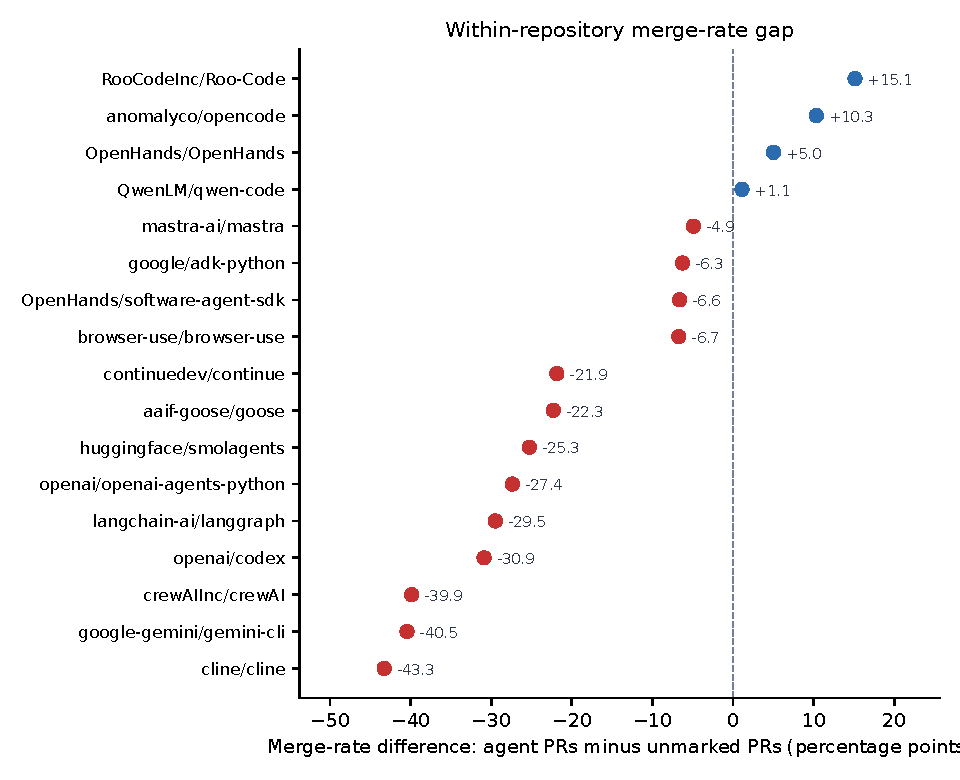
\includegraphics[width=0.72\textwidth]{figures/fig_merge_diff_en.pdf}
\caption{Within-repository difference in merge rate between explicitly agent-attributed PRs (T1+T2) and unmarked PRs. Negative values indicate that agent PRs are less likely to merge.}
\label{fig:merge}
\end{figure*}

Rework tells a weaker story. In the detail sample, median review counts are 0--2 for both agent and unmarked PRs in most repositories; the differences are not consistent in direction. In OpenCode, crewAI, and Gemini CLI, agent PRs receive fewer review comments; in Continue and Cline they receive more. We interpret this as a process effect---agent PRs may be triaged before review, or merged by the agent's own maintainers---rather than a quality effect.

Reverts are rare but skewed. T1 PRs are reverted at 0.33\% (7 of 2,141), T2 at 0.16\% (3 of 1,835), and T3 at 0.067\% (48 of 71,217). The T1 rate is about five times the baseline, but seven events cannot support a stable risk ratio. We report it as a signal, not an estimate.

\subsection{RQ2: Where do agent changes land?}

Table~\ref{tab:layers-dist} gives the weighted distribution of the primary layer. Autonomous agents are overwhelmingly concentrated in L4 (50.0\%), L0 (20.2\%), and LD (12.1\%). Only 2.4\% of T1 PRs have L1 as their primary layer, 1.0\% L2, and 5.1\% L3. Unmarked PRs are more evenly spread: 8.7\% L1, 2.8\% L2, 9.0\% L3, 40.5\% L4. Co-authored PRs sit between the two, with 3.5\% L1 and 10.7\% L3---higher than T1 in both cases.

\begin{table}[t]
\centering
\small
\caption{RQ2: weighted share of primary layer in the detail sample. Weights correct the intentional Tier-1 oversampling by repository--tier cell. Rows sum to about 90\%; the remainder is GEN, unclassified, or unknown.}
\label{tab:layers-dist}
\begin{tabular}{@{}lrrrrrr@{}}
\toprule
Tier & L1 & L2 & L3 & L4 & L0 & LD \\
\midrule
T1 & 2.4\% & 1.0\% & 5.1\% & 50.0\% & 20.2\% & 12.1\% \\
T2 & 3.5\% & 3.7\% & 10.7\% & 50.6\% & 11.9\% & 9.9\% \\
T3 & 8.7\% & 2.8\% & 9.0\% & 40.5\% & 17.4\% & 11.7\% \\
\bottomrule
\end{tabular}
\end{table}

The core-loop result is the cleanest evidence for a no-go zone. Weighted by repository--tier cell, 13.2\% of T1 PRs touch L1, versus 28.8\% of T2 and 26.0\% of T3. Combining T1+T2, the weighted odds ratio for touching the core versus T3 is 0.744 (bootstrap 95\% CI 0.614--0.864). The effect is not universal: software-agent-sdk's T1 PRs touch the core at 28.6\%, and Cline's T1 at 38.5\% (on 26 PRs), while crewAI's T1 is at 10.1\%. The boundary is set by repository policy, not by a fixed model capability.

Structural change follows the same split. T1 PRs are structural in 15.8\% of cases, T2 in 30.2\%, and T3 in 22.9\%. Autonomous agents are \emph{less} structural than the unmarked baseline; co-authored PRs are \emph{more} structural. This is consistent with a division of labor in which humans use agents to execute a design they already hold, while agents working alone make local repairs.

The abstraction-vs-patch adjudication points in the same direction but is weaker. Of 120 adjudicated PRs, 54 are conditional patches, 9 are abstraction extractions, 4 are mixed, and 53 are unclear. The 6:1 ratio is consistent with an entropy-accumulation story, but nearly half the sample is unclassifiable from a 2.5k-character patch excerpt, and the sample oversamples T1. We treat it as a directional signal.

\begin{figure*}[t]
\centering
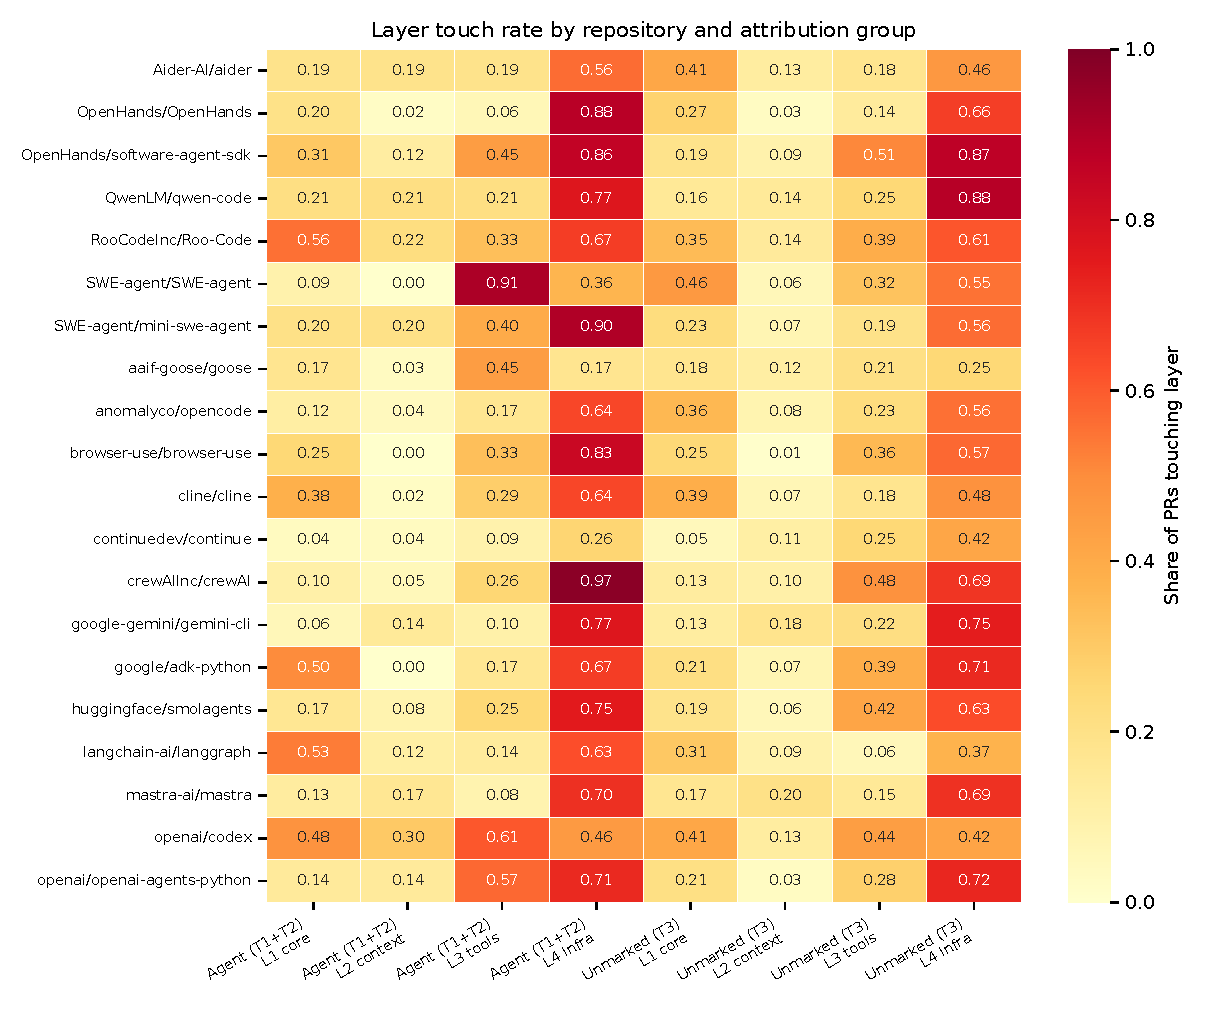
\includegraphics[width=0.92\textwidth]{figures/fig_layer_heatmap_en.pdf}
\caption{Repository-by-layer touch rates, agent-attributed versus unmarked PRs. Each cell is the share of PRs in that group touching the layer. L4 dominates agent activity in most repositories; L1 activity is sparse and repo-dependent.}
\label{fig:heatmap}
\end{figure*}

\subsection{RQ3: Diffusion and behavioral clusters}

We track six pattern families by keyword hits over PR titles and bodies. Table~\ref{tab:diffusion} shows the quarterly share of PRs mentioning each pattern. Skills/rules grows from 0.7\% in 2025Q2 to 12.7\% in 2026Q4; context compaction from 0.6\% to 5.8\%; sub-agents from 0.3\% to 4.8\%; checkpoints from 1.7\% to 5.9\%. MCP is already mature at the start (6.2\%) and grows modestly to 9.8\%. Diff/patch application declines from 0.9\% to 0.6\%.

\begin{table}[t]
\centering
\small
\caption{RQ3: quarterly share of PRs mentioning each pattern (percent of all merged PRs in the quarter).}
\label{tab:diffusion}
\begin{tabular}{@{}lrrrr@{}}
\toprule
Pattern & 2025Q2 & 2025Q4 & 2026Q2 & 2026Q4 \\
\midrule
Skills / rules & 0.7 & 1.5 & 7.7 & 12.7 \\
Context compaction & 0.6 & 1.6 & 4.1 & 5.8 \\
Sub-agent parallelism & 0.3 & 1.5 & 4.8 & 3.7 \\
Checkpoint / rollback & 1.7 & 0.9 & 2.3 & 5.9 \\
MCP integration & 6.2 & 5.9 & 8.4 & 9.8 \\
Diff / patch application & 0.9 & 0.9 & 1.0 & 0.6 \\
\bottomrule
\end{tabular}
\end{table}

The diffusion evidence is left-censored. MCP is present in 12 of 17 repositories at the first month of the window, and skills/rules in 5 of 18; for those cells we cannot identify first adoption, only intensity. The curves therefore describe how much change a pattern attracts, not when a repository first implemented it.

Who carries a pattern? Agent-attributed PRs are 5.6\% of MCP PRs, 4.9\% of compaction PRs, 7.8\% of sub-agent PRs, 4.0\% of diff/patch PRs, 3.9\% of checkpoint PRs, and 8.1\% of skills/rules PRs. The overall agent share is 5.2\%. There is no evidence that agents carry a disproportionate share of pattern diffusion; the ``humans invent, agents follow'' story is not supported by these counts, though it is not refuted either, because the pattern labels are lexical.

Finally, clustering repository--tier behavior vectors yields four clusters. A test-heavy cluster (L4 83\%, L1 18\%, structural 35\%) contains Qwen and OpenHands agent tiers. A core-heavy cluster (L1 44\%, L3 31\%, L0 28\%, structural 28\%) contains Aider, Roo-Code, SWE-agent, OpenCode's T2, and Cline. A tool-heavy cluster (L3 38\%, L4 75\%, L0 3\%, structural 14\%) contains software-agent-sdk, crewAI, browser-use, and mini-swe-agent. A mixed cluster (L1 15\%, L4 46\%, L0 42\%) contains the rest. Cluster membership is driven primarily by repository architecture; tier only creates substructure inside the test-heavy cluster. We read this as evidence that ``agent behavior'' is largely a function of the repository's architecture and review configuration, not of the agent's brand.

\begin{figure*}[t]
\centering
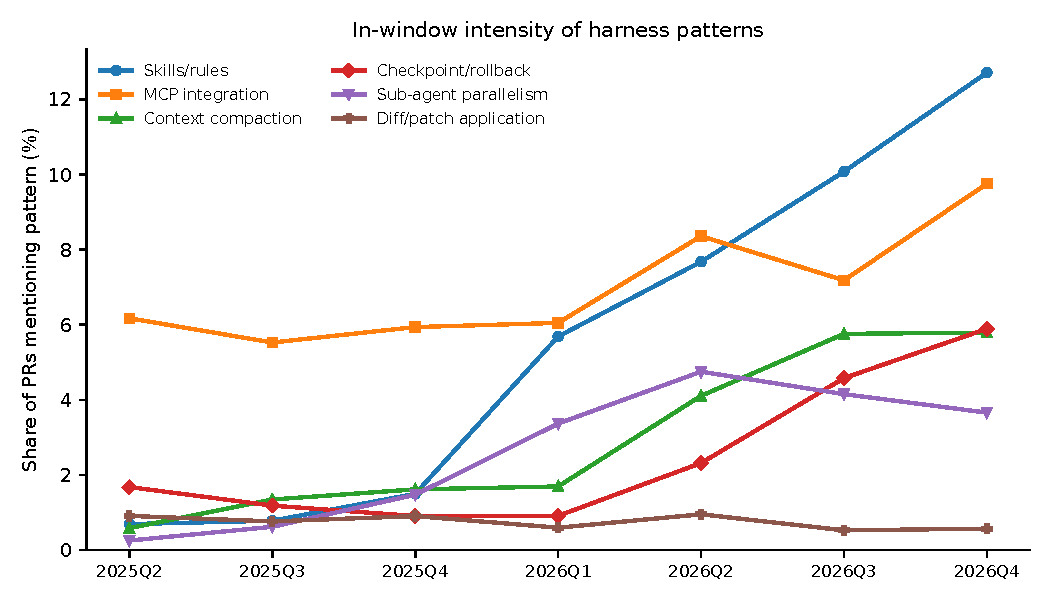
\includegraphics[width=0.88\textwidth]{figures/fig_diffusion_en.pdf}
\caption{Quarterly share of PRs mentioning each harness pattern. Patterns already present in 2025Q2 are left-censored; the curves measure change intensity, not confirmed adoption dates.}
\label{fig:diffusion}
\end{figure*}

\section{Discussion}
\label{sec:discussion}

\subsection{The variation seam is real, and it is where agents live}

The strongest pattern in our data is a division of labor by layer. Autonomous agents are concentrated in tests, infrastructure, UI, and documentation; they rarely own the core loop. Co-authored agents reach the core more often than unmarked PRs, and are more often structural. This is what a \emph{protected-variation} discipline looks like in practice: the stable core is closed to autonomous change, while the variation seam---adapters, tools, tests, prompts, UI---is open.

For object-oriented design, this is a useful empirical update. The classical advice ``program to an interface, not an implementation'' \citep{gof1994,parnas1972} predicts that agent labor should accumulate at interfaces and adapters. That is exactly what we observe: L3 tool/adapter work is 5.1\% of T1 primary layers and 10.7\% of T2, while L1 is 2.4\% and 3.5\%. The pattern vocabulary (Adapter, Strategy, Template Method, State, Proxy, Mediator) maps onto the layers where agents are actually productive and the layers where they are not.

\subsection{Design patterns for harness engineering}

Our results suggest three design rules for harness builders who expect agent contributors.

\textbf{Make the core contract explicit and mechanically checked.} If L1 is the no-go zone, its invariants should be executable: typed transition functions, contract tests, and negative controls that fail when an agent adds an unguarded branch. The rule engine's low L1 agreement ($\kappa=0.609$) is a warning: even expert instruments disagree about what counts as ``touching the core''. A harness that wants to delegate safely must define the pointcut precisely.

\textbf{Treat adapters and tests as the agent's native habitat.} L4 is the largest single layer for every tier, and T1 is nearly half L4. This is not a failure of ambition; it is the natural complement to a stable core. Harness designs that isolate provider adapters, tool schemas, and test fixtures behind narrow interfaces will get more value from agent contributions and fewer merge conflicts.

\textbf{Route co-authored work through the core.} T2 is the only group that touches L1 more often than the baseline and is structural more often than the baseline. The practical implication is that the co-authored path---human holds the design, agent executes---is the mechanism by which agents participate in architecture. Organizations that want architectural RSI should invest in that path, not in fully autonomous PRs.

\subsection{Governance dominates agent brand}

The merge-rate heterogeneity ($+15$ to $-43$ percentage points) is too large to be a model-quality effect. It aligns with repository policy: whether agent accounts are allowlisted, whether their PRs bypass triage, whether maintainers review them like human PRs. This echoes the pull-based development literature: contribution outcomes depend on social and technical signals, not only on the diff \citep{tsay2014,gousios2014}. For RSI research, the implication is that ``agent capability'' studies that pool repositories will estimate a mixture of governance regimes and report an uninterpretable average.

\subsection{RSI as maintenance-layer self-improvement}

The data support a modest version of RSI. Agents do write to their own harness: 5.2\% of PRs are explicitly attributable, and in some repositories the share is above 10\%. But the self-improvement is concentrated in maintenance layers. The core loop, the permission model, and the concurrency architecture remain human-authored. This is not a failure of the RSI hypothesis; it is a specification of its current scope. The interesting question for the next period is whether the boundary moves when contract tests and sandboxed execution make L1 changes safer to delegate. The benchmark results of Harness$^2$ and OO-Harness show that harness-level improvement is technically feasible \citep{xu2026harness2,li2026ooharness}; our mining results show that, in the wild, it is still concentrated in maintenance layers.

\section{Threats to Validity}
\label{sec:threats}

\textbf{Construct validity.} Tier~3 is an unmarked baseline, not a pure-human control. Unmarked AI assistance (copy-paste from Cursor or Claude Code) contaminates it and biases agent effects toward zero. Tier~2 is undercounted in the census because commit trailers are only visible in the 7,205-PR detail sample; the 2.33\% share is a lower bound. The layer taxonomy is path-based and cannot see semantic coupling: a one-line change to a shared type may alter the loop without touching an L1 path. The model-assisted adjudication is not human double-coding; its $\kappa$ values (0.566 for change type, 0.579 for core touch) are below our thresholds, so layer conclusions carry 10--20 percentage points of classification uncertainty.

\textbf{Internal validity.} The detail sample intentionally oversamples T1; weighted estimates correct the quantity but not the composition of agent types. Same-lineage repositories (Cline/Roo-Code, Gemini CLI/Qwen Code, OpenHands/software-agent-sdk) are not independent, so pooled confidence intervals are too narrow; we rely on within-repository comparisons and report the lineage pairs explicitly. OpenHands cleared its Python backend on 2026-07-27; after that date its core-layer PRs live in software-agent-sdk. We break the time series at that point and do not sum the two repositories. Roo-Code (archived 2026-05), Continue (dormant 2026-07), and SWE-agent (dormant 2026-07) are right-censored at their last activity.

\textbf{External validity.} The sample covers 20 repositories and one forge (GitHub) in one 18.6-month window. It over-represents TypeScript and Python and under-represents industrial closed-source harnesses. The findings describe the open-source frontier of 2025--2026, not a universal law of agent-assisted evolution.

\textbf{Conclusion validity.} Merge rate is not quality; a lower merge rate can reflect stricter review, a different contributor mix, or a backlog. Reverts are identified only by explicit revert markers, so the T1 revert rate is a lower bound with seven events. Pattern detection is lexical and left-censored; the diffusion curves measure attention and change volume, not confirmed adoption. Multiple repository-level tests are corrected with Benjamini--Hochberg, but the layer and change-type comparisons are exploratory and should be replicated.

\section{Conclusion and Future Work}
\label{sec:conclusion}

We studied 135,331 pull requests across 20 open-source agent harnesses to ask who rewrites the harness, where, and with what success. Explicit agent attribution is 5.2\%; agent PRs merge less often overall (OR 0.709) but the effect reverses in repositories that treat agents as first-class contributors. Autonomous agents are concentrated in tests, infrastructure, UI, and documentation: 13.2\% touch the core loop versus 26.0\% of unmarked PRs, and 15.8\% are structural versus 22.9\%. Co-authored PRs are the exception: they touch the core at 28.8\% and are structural at 30.2\%, making human--agent pairing the main channel for architectural change.

The design implication is a protected-variation discipline for harness engineering: define the core contract, mechanize its tests, open the adapter and test seams, and route co-authored work through the core. The research implication is that RSI should be measured as a layer-specific spectrum, with governance as a first-class variable, rather than as a binary claim about agent capability.

Future work should replicate the taxonomy on closed-source and non-GitHub harnesses, add AST-level refactoring detection to replace the proxy metrics, obtain true human double-coding for the adjudication set, and track whether the L1 boundary moves as contract tests and sandboxed execution mature.

\section*{Data Availability}

The cleaned census (135,331 PRs), the 7,205-PR detail sample, the labeling specification, the taxonomy, and the analysis scripts are available in the replication package. The raw database is 506 MB; the CSV exports are 5.5 MB and 439 KB compressed.

\begin{thebibliography}{99}
\small

\bibitem[Barke et al.(2023)]{barke2023}
S.~Barke, M.~B. James, and N.~Polikarpova.
\newblock Grounded {Copilot}: How developers interact with {AI} code generators in {IDE}s.
\newblock \emph{Proc. ACM Program. Lang.} (OOPSLA), 2023.

\bibitem[Benjamini and Hochberg(1995)]{bh1995}
Y.~Benjamini and Y.~Hochberg.
\newblock Controlling the false discovery rate: A practical and powerful approach to multiple testing.
\newblock \emph{Journal of the Royal Statistical Society: Series B}, 57(1):289--300, 1995.

\bibitem[Bird et al.(2009)]{bird2009}
C.~Bird, P.~C. Rigby, E.~T. Barr, D.~J. Hamilton, N.~Nagappan, and A.~Devanbu.
\newblock The promises and perils of mining {Git}.
\newblock \emph{Proc. MSR}, 2009.

\bibitem[Chen et al.(2021)]{chen2021}
M.~Chen, J.~Tworek, H.~Jun, et al.
\newblock Evaluating large language models trained on code.
\newblock \emph{arXiv:2107.03374}, 2021.

\bibitem[Cohen(1960)]{cohen1960}
J.~Cohen.
\newblock A coefficient of agreement for nominal scales.
\newblock \emph{Educational and Psychological Measurement}, 20(1):37--46, 1960.

\bibitem[Fielding(2000)]{fielding2000}
R.~T. Fielding.
\newblock \emph{Architectural Styles and the Design of Network-based Software Architectures}.
\newblock PhD thesis, University of California, Irvine, 2000.

\bibitem[Fowler(2018)]{fowler2018}
M.~Fowler.
\newblock \emph{Refactoring: Improving the Design of Existing Code}, 2nd edition.
\newblock Addison-Wesley, 2018.

\bibitem[Gamma et al.(1994)]{gof1994}
E.~Gamma, R.~Helm, R.~Johnson, and J.~Vlissides.
\newblock \emph{Design Patterns: Elements of Reusable Object-Oriented Software}.
\newblock Addison-Wesley, 1994.

\bibitem[Godfrey and German(2008)]{godfrey2008}
M.~W. Godfrey and D.~M. German.
\newblock The past, present, and future of software evolution.
\newblock \emph{Proc. Frontiers of Software Maintenance}, 2008.

\bibitem[Gousios et al.(2014)]{gousios2014}
G.~Gousios, M.~Pinzger, and A.~van Deursen.
\newblock An exploratory study of the pull-based software development model.
\newblock \emph{Proc. ICSE}, 2014.

\bibitem[Herbsleb and Mockus(2003)]{herbsleb2003}
J.~D. Herbsleb and A.~Mockus.
\newblock An empirical study of speed and communication in globally distributed software development.
\newblock \emph{IEEE Transactions on Software Engineering}, 29(6):481--494, 2003.

\bibitem[Jimenez et al.(2024)]{jimenez2024}
C.~E. Jimenez, J.~Yang, A.~Wettig, S.~Yao, K.~Pei, O.~Press, and K.~Narasimhan.
\newblock {SWE-bench}: Can language models resolve real-world {GitHub} issues?
\newblock \emph{Proc. ICLR}, 2024.

\bibitem[Kalliamvakou et al.(2014)]{kalliamvakou2014}
E.~Kalliamvakou, G.~Gousios, K.~Blince, L.~Singer, D.~M. German, and D.~Damian.
\newblock The promises and perils of mining {GitHub}.
\newblock \emph{Proc. MSR}, 2014.

\bibitem[Lehman(1980)]{lehman1980}
M.~M. Lehman.
\newblock Programs, life cycles, and laws of software evolution.
\newblock \emph{Proceedings of the IEEE}, 68(9):1060--1076, 1980.

\bibitem[Li et al.(2026)]{li2026ooharness}
G.~Li, B.~Dalvi Mishra, Y.~Ming, Y.~Chen, Z.~CuiZhu, L.~Miculicich, L.~T. Le, R.~Meng, C.-L. Li, H.~Tong, C.-Y. Lee, and T.~Pfister.
\newblock Object-oriented harness: Evolving agent harnesses through object-oriented design.
\newblock \emph{arXiv:2610.28380}, 2026.

\bibitem[Mantel and Haenszel(1959)]{mantel1959}
N.~Mantel and W.~Haenszel.
\newblock Statistical aspects of the analysis of data from retrospective studies of disease.
\newblock \emph{Journal of the National Cancer Institute}, 22(4):719--748, 1959.

\bibitem[Mockus et al.(2002)]{mockus2002}
A.~Mockus, R.~T. Fielding, and J.~D. Herbsleb.
\newblock Two case studies of open source software development: {Apache} and {Mozilla}.
\newblock \emph{ACM Transactions on Software Engineering and Methodology}, 11(3):309--346, 2002.

\bibitem[Nagappan et al.(2008)]{nagappan2008}
N.~Nagappan, B.~Murphy, and V.~Basili.
\newblock The influence of organizational structure on software quality: An empirical case study.
\newblock \emph{Proc. ICSE}, 2008.

\bibitem[Parnas(1972)]{parnas1972}
D.~L. Parnas.
\newblock On the criteria to be used in decomposing systems into modules.
\newblock \emph{Communications of the ACM}, 15(12):1053--1058, 1972.

\bibitem[Peng et al.(2023)]{peng2023}
S.~Peng, E.~Kalliamvakou, P.~Cihon, and M.~Demirer.
\newblock The impact of {AI} on developer productivity: Evidence from {GitHub Copilot}.
\newblock \emph{arXiv:2302.06590}, 2023.

\bibitem[Rigby et al.(2008)]{rigby2008}
P.~C. Rigby, D.~M. German, and M.-A. Storey.
\newblock Open source software peer review practices: A case study of the {Apache} server.
\newblock \emph{Proc. ICSE}, 2008.

\bibitem[Schmidt et al.(2000)]{posa2000}
D.~Schmidt, M.~Stal, H.~Rohnert, and F.~Buschmann.
\newblock \emph{Pattern-Oriented Software Architecture, Volume 2: Patterns for Concurrent and Networked Objects}.
\newblock Wiley, 2000.

\bibitem[Tsantalis et al.(2022)]{tsantalis2022}
N.~Tsantalis, A.~Ketkar, and D.~Dig.
\newblock {RefactoringMiner} 2.0.
\newblock \emph{IEEE Transactions on Software Engineering}, 48(1):1--20, 2022.

\bibitem[Tsay et al.(2014)]{tsay2014}
J.~Tsay, L.~Dabbish, and J.~Herbsleb.
\newblock Influence of social and technical factors for evaluating contribution in {GitHub}.
\newblock \emph{Proc. ICSE}, 2014.

\bibitem[Wang et al.(2025)]{wang2025}
X.~Wang, B.~Li, Y.~Song, et al.
\newblock {OpenHands}: An open platform for {AI} software developers as generalist agents.
\newblock \emph{Proc. ICLR}, 2025.

\bibitem[Xu et al.(2026)]{xu2026harness2}
R.~Xu, Y.~Chen, Z.~CuiZhu, B.~Dalvi Mishra, Y.~Ming, H.~Yu, R.~Han, C.-Y. Lee, and T.~Pfister.
\newblock {Harness}$^2$: Recursive agent harnessing for an open world.
\newblock \emph{arXiv:2610.14224}, 2026.

\bibitem[Yang et al.(2024)]{yang2024}
J.~Yang, C.~E. Jimenez, A.~Wettig, K.~Lieret, S.~Yao, and O.~Press.
\newblock {SWE-agent}: Agent--computer interfaces enable automated software engineering.
\newblock \emph{Proc. NeurIPS}, 2024.

\bibitem[Ziegler et al.(2022)]{ziegler2022}
A.~Ziegler, E.~Kalliamvakou, X.~A. Li, A.~Rice, D.~Rifkin, S.~Simister, G.~Sittampalam, and E.~Aftandilian.
\newblock Productivity assessment of neural code completion.
\newblock \emph{Proc. MAPS}, 2022.

\end{thebibliography}

\end{document}
